\chapter{Introduction} \label{introduction} 

The purpose of this research is to make a contribution in the
application of contextual information in recommender systems by
proposing a methodology for the development of context aware
recommender systems. The method follows an hybrid  approach by
integrating several recommendation techniques through a fuzzy
inference system. The proposed method was validated by the
execution of several experiments, and the implemantion of a case
study. The results presented are favorable, indicating the
strenghts of the hybrid method.

\section{Motivation}

Often people need to take decisions, even when they do not
have enough experience or information to discern among 
the possible alternatives. For this, is common for people to 
seek help by asking friends  or people which they  
have certain level of affinity for their recommendations.\\
The problem of making a decision is aggravated by the 
large amount of information generated by society, 
resulting in an information overload where users are not capable of
sorting out the relevant information from the irrelevant.
This lack of experience, time and other resources 
highlights the need of automatic or semi-automatic methods 
to filter relevant information. Currently, information filters are
an integral component of the Web, where for instance
automatic search engines help users to find or make 
decisions through (some times) personalized recommendations
of products and services. \\ On the other hand, in recent
years  mobile computing has drasticaly incremented their importance, 
because of the impact of their use in daily life, if an application 
is available in a smartphone it can be used all most anywhere, and thanks
to sensors and GPS technology location aware applications are now common.\\ 
New technologies also consider information about the user's current situation 
in mobile applications, as intelligent systems can take advantage of the
benefits that this technology provides, to manage the constantly changing 
context. \\ Developments in mobile and ubiquitous computing \cite{noguera2012mobile} 
\cite{chiou2010adaptive}, are proposing a wide variety of applications
that will benefit from recommendation engines using context to meet their
purpose. But still there is a need to model the information available in
the system in order to provide context awareness.\\  Information regarding 
context can also be described in natural language in a fuzzy manner. For
instance when describing the current situation an user could say: \textit{``Is early in
the morning and I am currently near my work and I need to find a coffee
shop that is not to expensive, is open and not very far"}.
This sentence uses many words to describe the situation that are not 
crisp, but instead, the description uses fuzzy variables to describe the situation.  

\section{Context of use}\label{contextofuse}

Context is an important concept in everyday life. People often provide
context when writing postcards, referring to the weather or the holiday
atmosphere. A knowledge of context can also help to explain why a certain
object is produced or designed the way it is. When a product 
(or system) is developed, it
will be used within a particular context. It will be used by a user
population with certain characteristics. The user will have certain
goals and has the intension to perform certain tasks. The product will also be used
within a certain range of technical, physical and social or
organizational environments \cite{maguire2001context} that may affect
its use.\\   
We can refer to these environments as the \textit{context of use} (see
Figure \ref{fig:logicalmodel}), this concept has been formally defined
by ISO standard 9241-11 \cite{international1998iso} as \textit{``users,
tasks and equipment (hardware, software and materials), and the
physical and social environments in which a product is used"}. \\ 
In daily life we often find products that are difficult to use or
understand. This type of difficulties are \textit{usability problems}
that arise from  diverse issues that have not been addressed in the
design of the product's \textit{user-artifact interaction}. The
\textit{user-artifact interaction} refers the way that the user
interacts with a product and vice versa, this term has been studied
in Human Computer Interaction. \\As emerging technologies constantly
change the way people interact with products and their physical
environment, recent studies have started looking at \textit{human
experience} as a source to generate products or systems that
\textit{engage} the user.\\
The \textit{user experience}, \textit{context of use} and
\textit{product usability} have been associated in computer sciences
field. The \textit{Usability} is became a well-established concept in
the IT world to represent the user-friendliness of a system. However,
there was a need to establish the concept more clearly and to
determine how to measure it. Probably the best known definition of
usability is by Nielsen \cite{nielsen1994usability}: 
\textit{``usability is about learnability, efficiency, 
memorability, errors, and satisfaction".}
However, the definition of usability from ISO
9241-11 \cite{international1998iso}:\textit{``the extent to which a
product can be used by specified users to achieve specified  goals
with effectiveness, efficiency and satisfaction in a  specified
context of use"}, is becoming the main reference of usability. \\
Thus, taking in account these definitions we can say that designing for 
\textit{usability} involves establishing user requirements for a new
\textit{system} or \textit{product}, developing design solutions,
prototyping the system and the user interface, and testing it with
representative users.\\
In the study of Sato \cite{sato2004context} that brings \textit{context
issues} into design practice, addressed the concept of
\textit{context} as a critical component of the design information in
order to enhance the \textit{human-centred design practice}. After a
literature's revision for  definitions of \textit{context} in diverse
fields, Sato explains that there are external and internal conditions
into the definitions and suggest that it has four characteristics:
\begin{enumerate}  
\item Aspects of context are based on the nature of actions and 
conditions.
\item Descriptions depends on the focus of the viewpoints.
\item Contextual changes are triggered from differents elements 
of the domain. 
\item Context evolves over the time, some aspects change fast
and others change slow. 
\end{enumerate} 
From this, Sato defined \textit{context} as a \textit{mental model} or a
\textit{pattern of one's memory} triggered by \textit{elements in the
situation}, where situation is a collective condition at the scene of
interaction composed of relations among \textit{variables of
conditions}. Sato employed this concept to describe the
\textit{influence of contexts} in \textit{people's interactions} and
\textit{system performance} and vice versa.

\subsection{Logical model of context} 

The \textit{logical model} explains the relationship between \textit{context},
\textit{contextual information} and \textit{contextual factors}. 
Figure \ref{fig:logicalmodel} gives a graphical representation of these relations. 
The goal is to facilitate the use and implementation of fuzzy context 
in recommender systems for different domains.\\
In the Figure \ref{fig:logicalmodel}, the first box shows different
real life situations of the user (contexts), the user can change from situation
to situation in a little time or in a long time, this situational or
contextual information in the real world provides the abstract knowledge that
the system will use to determine the \textit{``contextual information"} that will 
be used. 
From the real world, specific data will be extracted by different means as
sensors, user interaction or even manual input. In this work 
we call this data \textit{``contextual factors"}(for instance, place and
orientation, preferences, date and time, etc.) and represent the
information that affects the recommendation process. The information
could be represented as fuzzy variables or crisp variables depending of
its domain. Later, contextual factors are implemented as data
structures that define the domain for each one. 
%\begin{landscape} 
\begin{figure*}
\captionsetup{font=footnotesize} \centering
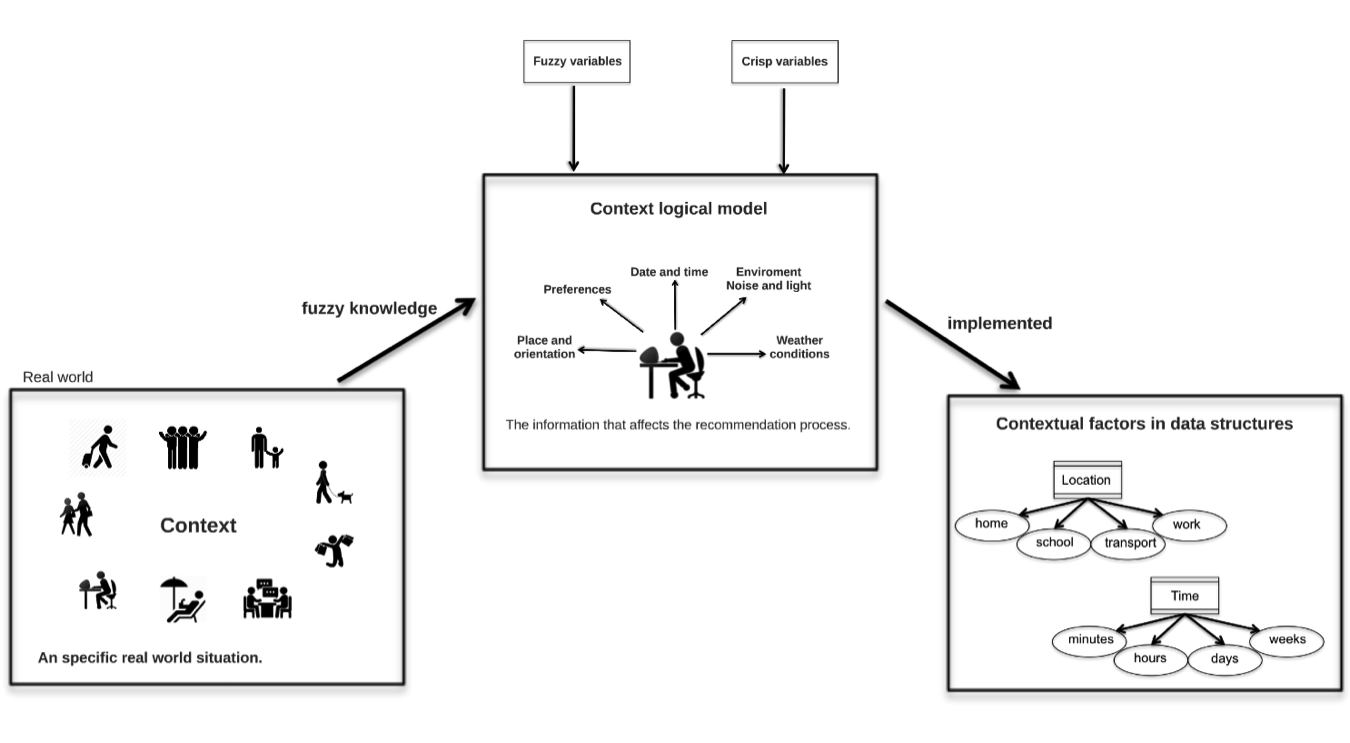
\includegraphics[width=1.0\textwidth]{img/context-scheme.png}  
\small
\caption{Logical data model of context.}
\label{fig:logicalmodel}    
\end{figure*} %\end{landscape}

\section{Context-awareness} \label{context-awareness}

Traditional recommender systems provide suggestions of useful items
for a certain user. The suggestion relates to various decision-making
processes, for instance, what items to buy, what music to listen to, or
what on-line news to read. \textit{Item} is the general term to denote
what product or service the system recommends for each user. A
recommender system normally focuses only on a single type of item
 \cite{resnick1997recommender}.
Some improvement efforts for recommender systems, have been mainly
focused on the
\textit{integration of context} in the recommendation process. 
The idea behind \textit{context-aware computing} is to provide
information or services for the user based in the user's situation
 \cite{dey2001understanding}. In order to do that, the application 
needs to obtain situational data, process it, and make use of it 
in a manner that benefits the user. \\ 
\textit{Context} is a concept that is not easy to define, as it is related with
several disciplines that propose different definitions. For example,
the authors Bazire et.al. \cite{bazire2005understanding} compare the
notion of context in different fields and conclude that is complicated to make a
unifying definition of context because of the nature of the concept in
many disciplines. In computer science Fischer \cite{fischer2012context}
defines context as \textit{``the interaction between humans and
computers in socio-technical systems that takes place in a certain
context referring to the physical and social situation in which
computational devices and environments are embedded"}. 
Fischer also identifies
the important aspects to consider when the context is used: how it is
the contextual data obtained, how the context is represented and what
goals and purposes the context has when is used in a particular
application. \\
Probably the definition most used in the field of recommender systems to 
define \textit{context} is proposed by Dey \cite{dey2001understanding}:
\textit{``Context is any information that can be used to characterize
the situation of an entity. An entity is a person, place or object
that is considered relevant to the interaction between a user and an
application, including the user and applications themselves.''}  This
definition makes it easier to define the contextual factors in a
specific application. For instance, in a tourist guide application, the
entities can be companion(friends, family, couple), place of interest,
season and weather, these could be considered as relevant contextual
factors that help the recommender system to provide items adjusted the
situational data of the user.\\
\textit{Context-aware recommender systems} are gaining even more
attention because of their performance and implementation for
different domains, the  way to improve personalized recommendations
based in contextual factors is an important technique to increase the
benefits in  many domains. For instance, taking in account the
\textit{hour of the day},  or the \textit{day of the week} when
recommending restaurants could  filter out restaurants that are
currently closed or near closing time, when the user receives this
information in real time, the user has the  way for taking
alternatives of restaurants that provide services. Nowadays, many
companies are incorporating some type of context (as time, location or
companion) in their recommendation engines, the application can be
found in fields such as e-commerce \cite{schafer1999recommender}
 \cite{bulander2005enabling}, music \cite{ricci2012context}
 \cite{baltrunas2011incarmusic}  \cite{huq2010automated}, places of
interest \cite{baltrunas2012context},
movies \cite{eyjolfsdottir2010moviegen}, vacation
packages \cite{liu2011personalized}  \cite{liu2014cocktail},  travel
guides \cite{savage2012m}, e-learning \cite{ortigosa2010entornos}  and
restaurants \cite{chu2013chinese}.\\
Plus, context can be used to improve the user satisfaction  in
recommender systems, thus the quality and accuracy of predictions  
is improved too. \\
The method proposed in this thesis uses three recommendations techniques,
applied as a case study in a restarant domian:
\begin{enumerate} 
\item \textit{Expert's Fuzzy Inference System}, this is a rule based 
recommender defined by an expert in the domain, in the case of 
a restaurant recommender, it considers the following
variables: \textit{ratings average: low,medium and high},
\textit{price of restaurant: cheap, average and expensive}, and
\textit{number of ratings of item: few, several and many}, these
variables are used to infer how relevant a restaurant is, for the user.
This recommendation is based on the popularity of each item in the
user's community.
\item \textit{Content-based technique} utilizes the item profiles 
to compare how \textit{similar} is an item with respect to 
another, i.e. restaurants that are \textit{similar} (same cuisine, 
ambient, price range) to others that the user has rated high. 
The idea is to find items with similar features. 
\item \textit{Collaborative filtering technique} is based on the user
profile to identify user's preferences and to find neighbors that
have the same tastes. The recommendation consist in the suggestions of
other users with similar tastes that rated restaurants again in a
similar way but where have not been rated by the current user. A Top-N
list of restaurants is obtained to recommend for the user.
\end{enumerate} 
The results of the three techniques are a list of recommendations for
the user, later, these recommendations are adjusted for the current context.
This is the last step and is represented as a \textit{context filter} in the
method, as a result a list of contextualized
recommendations is obtained. \\
In the method, each technique works simultaneously to obtain
recommendations, the hybrid method allows to generate suggestions even
without user information, i.e., using content-based technique or the
fuzzy inference system, so the system faces the cold-start or the
overspecialization problem using these thechniques, these problems are
described in section \ref{coldstart} and 
 \ref{overspecialization}, respectively.\\
To evaluate the performance of the proposed recommender several experiments
were maded, the algorithms were tested using contextual datasets and
the number of contextual factors used varied according to the information
provided by the dataset. The goal of the experiments were to observe
the role of contextual data  in the performance of the algorithms and to 
have a better understanding of what contextual
factors are more important for users in a specific situation, how recommendations
are improved using context and, the accuracy in recommendations.
Chapter 5 shows the results while discussion about results are
explained in each section.\\
As a user-cenetered system another important aspect 
to consider and measure is the \textit{user satisfaction}, for this two
metrics were used: \textit{task-success} and \textit
{time-on-task}. These usability metrics allow designers to measure 
the user experience.
\\ Usability
metrics can help reveal patterns that are hard or even impossible to
see. Evaluating software applications with a small sample size 
(between 5 and 8 tests) usually reveals the most obvious 
usability problems \cite{albert2013measuring}.\\ 
Then, as
a general rule of thumb, during the early stages of design, it needs
fewer participants to identify the major usability issues. As the
design gets closer to completion, the tests should include more
participants to identify the remaining
issues \cite{albert2013measuring}.\\ 
Following this precept, ten representative users were selected to test
the system, subsequently, it was realized an analysis about the system
performance and issues presented in the user interaction. The chapter
6 explains the process to evaluate the system and the
results obtained.

\section{Aims}

Recommender systems has been used to obtain relevant items for current user
through simple models (user-item), the technique is limited 
because of ignore information about behaviour of users and others
factors that are involved in the user environment. 
To implement new tecnologies to adapt
the recommender algorithms for the user needs is the novel approach in
recommender systems. 
The purpose of them is to improve the suggestions in order to increase the user
satisfaction as well as to facilitate the interaction user-system.
The improves proposed by researchers in this field involve the context
implementation, through contextual factors defined according the domain 
proposed, and considering 
experiences and recommendations of other authors.
The goal of this thesis highliths the implementation of context in 
a method that includes fuzzy logic
techniques and pre-filtering paradigm that uses traditional recommender
techniques improved to make recommendations. To achieve this, 
uses of fuzzy rules to treat linguistic terms that include fuzzy variables, 
this allows the use of aproximated information 
to the real context of the user, and it allows an improved
performace of the recommender system because analyzes the user 
preferences and obtain recommendations
based in contextual factors. 
For instance, the system provides a list of
range of prices, this allows the users to select a specific range of
price to get recommendations adjusted for the tag selected, this tag represents
a common word of their native language.\\
The contribution of this thesis is the novel method that 
includes a hybrid recommender
system (content-based and collaborative filtering techniques). It
provides a \textit{useful knowledge} 
to utilize in the hybrid recommender system, provides techniques to 
maximize the use of context by fuzzy variables that represent a part
of context. The context complementation is represented by external factors
such as web services. 
Plus, the method has features that allow to adapt it to be
implemented in different domains such as e-learning, movies,
music, tourism, etc. For a case of study, the restaurants domain
was used to test the method.\\
Several particular aims were done in order to support the achievement 
of contributions:
\begin{itemize}  
\item Elaborate an analysis about the state of the art in the field
of context-aware recommender systems through  the revision of 
the relevant literature. State of the art helps to define the tendency
of currents recommender systems, the recent improves and helps to understand
what is the relevance of the proposed method as well as the factibility and 
how we can make an important contribution to the recommender systems field.
\item Selection of algorithms that are representative of the alternatives for
this problem domain in order to compare their perfomance. An analisys of the 
features and performs of the algorithms was done, it was extracted of papers,
books, and toolbox results to choose the suitable algorithm
for the method. There are enough papers to make a consense about 
what is that we want from each one. 
\item Design and conduct several experiments with the proposed 
algorithms. The experiments were based in previous results of similar 
methods, the algoritms were adjusted to improve their performance and 
testing with datasets for several applications, such as travels, hotels, 
restaurants and movies. The  metric implemented to measure the experiments 
results was root mean square error beause of is the most recommended 
by literature.
\item Propose a hybrid method and apply it in a case of study. 
Subsequently the results obtained, the proper algorithms and paradigm was 
included in the proposed method. As well as the fuzzy inference system and 
the fuzzy variables to represent the context used by the 
recommender system.
\item Develop a prototype of a context-aware recommender system 
using the proposed method. Using recent technologies to develop a proper 
interface for restaurant recommender system as case of study, 
the development was done to apply the proposed method. The 
context is represented by fuzzy variables and database models 
related the user model and characteristics
that describe the restaurant model.
\item To evaluate the proposed method the usability metrics were proposed. 
We consider the nature of the recommender system and the results 
that we can get of usability test. The test was prepared to be realized
by real users that never have been interacting with recommender systems. 
Results are explained in a posterior chapter.
\end{itemize} 

\section{Outline}

The rest of this thesis is organized as follows: 
\begin{itemize}  
\item \textbf{Chapter 2} describes an in-depth study
and background of current and related work, presenting a general
overview of recommender systems and their evolution in recent years.
This study includes traditional recommender systems, their methods
and techniques to improve recommendations, aswall as the challenges 
of these systems. Subsequently, hybrid methods used in different
applications, their limitations and advantages for each hibridation and
the domains of application. Finally, context-aware recommender systems
are disscussed, in the same way,  with an analysis of the advantages and
disadvantages of the use of context in recommender systems.
\item \textbf{Chapter 3} describes the fundamental
concepts that form the basis of the proposed method.
\item \textbf{Chapter 4} presents a model of context-aware
recommender system, the proposed method involves the paradigm of
post-filtering in a restaurants domain. This chapter includes the
overall explanation of data models and  the functionality, as
well as its components for this case of study.
\item \textbf {Chapter 5}, the general results of different
projects involved are presented along with the validation of every
experimentation. The experiments were realized using different
datasets and different algorithms in order to find an optimal manner
to reduce the error level. This chapter also details the results for
each experiment from a point of view of scientific results.
\item \textbf {Chapter 6}, after the development of
context-aware recommender system, the impact of
context in recommendation process was evaluated. 
This chapter describes the
usability tests that were applied on-line in order to evaluate the
satisfaction of users. Details of the environment and the
characteristics of the tests are described, as well as 
the results of each one.
\item \textbf {Chapter 7}, this chapter concludes with a
summary of its contributions and limitations. Final
conclusions are drawn and also proposals for future work are presented.
\end{itemize}  
At the end, this thesis includes appendices that describe
detailed technical aspects about installation and libraries of python
that uses the context-aware recommender system  \textit{(appendix \ref{appendixa})}, 
the pseudocode of algorithms proposed in the method are available in  \textit{(appendix \ref{appendixb})}, 
and experiment study materials used to obtain the test results are in  \textit{(appendix \ref{apendixc})}.
